\chapter{What Is Respiration?}\label{ch:g7:what-is-respiration}

Put a woodlouse in a closed jar and, hours later, the air in
the jar has changed: some of its \omterm{def:g7:what-is-respiration:respiration}{oxygen} is gone, replaced by
\omterm{def:g7:what-is-respiration:respiration}{carbon dioxide}. Repeat with a germinating \omterm{def:g2:from-seed-to-plant:seed}{seed}, a mushroom, a
goldfish, a spoonful of living \omterm{def:g6:decomposers-and-soil:soil}{soil} --- same result, every
time. \Cref{prop:g4:breathing:exchange} showed the swap in
your own chest; this year opens the idea to its full width:
the swap is not a human habit but a property of life itself.

\section{Respiration, defined and measured}

\begin{definition}[Respiration]\label{def:g7:what-is-respiration:respiration}
\emph{Respiration}\index{respiration} is the gas exchange by
which a \omterm{def:g6:exploring-our-environment:components}{living thing} takes \emph{oxygen}\index{oxygen} from
its surroundings and releases \emph{carbon
dioxide}\index{carbon dioxide}. It must not be confused with
\emph{breathing}\index{breathing} --- the visible chest
movements of \cref{def:g4:breathing:movements}: breathing is
one way of \emph{serving} respiration; respiration itself is
the gas swap, and it goes on in every living \omterm{def:g5:first-look-at-cells:cell}{cell}, movements
or none.
\end{definition}

\begin{proposition}[How the swap is shown]\label{prop:g7:what-is-respiration:shown}
Two standard bench tests reveal \omterm{def:g7:what-is-respiration:respiration}{respiration}:
\begin{itemize}
  \item an \emph{\omterm{def:g7:what-is-respiration:respiration}{oxygen} probe} in a closed container shows
        the \omterm{def:g7:what-is-respiration:respiration}{oxygen} level falling while a \omterm{def:g6:exploring-our-environment:components}{living thing} sits
        inside;
  \item \emph{limewater}\index{limewater}, a clear liquid
        that turns milky in \omterm{def:g7:what-is-respiration:respiration}{carbon dioxide}, clouds when the
        container's air is passed through it.
\end{itemize}
Falling \omterm{def:g7:what-is-respiration:respiration}{oxygen} plus clouding \omterm{prop:g7:what-is-respiration:shown}{limewater}, with a lifeless
control container staying unchanged
(\cref{met:g4:what-plants-need:fairtest} --- the fair test
follows us everywhere): that is \omterm{def:g7:what-is-respiration:respiration}{respiration}, measured.
\end{proposition}
\admitted

\begin{example}[The gallery of respirers]\label{ex:g7:what-is-respiration:gallery}
Run the two tests on a menagerie: a mouse --- fast fall,
quick clouding; a woodlouse --- the same, smaller; a
germinating pea --- unmistakable (a jar of sprouting peas
can exhaust its \omterm{def:g7:what-is-respiration:respiration}{oxygen} in a day); a mushroom --- yes; pond
snails --- yes; a spoonful of living \omterm{def:g6:decomposers-and-soil:soil}{soil} --- yes, its
billions of \omterm{def:g6:decomposers-and-soil:decomposers}{decomposers} respiring together
(\cref{ex:g6:decomposers-and-soil:handful}). Only the
control jar --- pebbles, dry sand --- changes nothing.
\end{example}

\begin{omfigure}
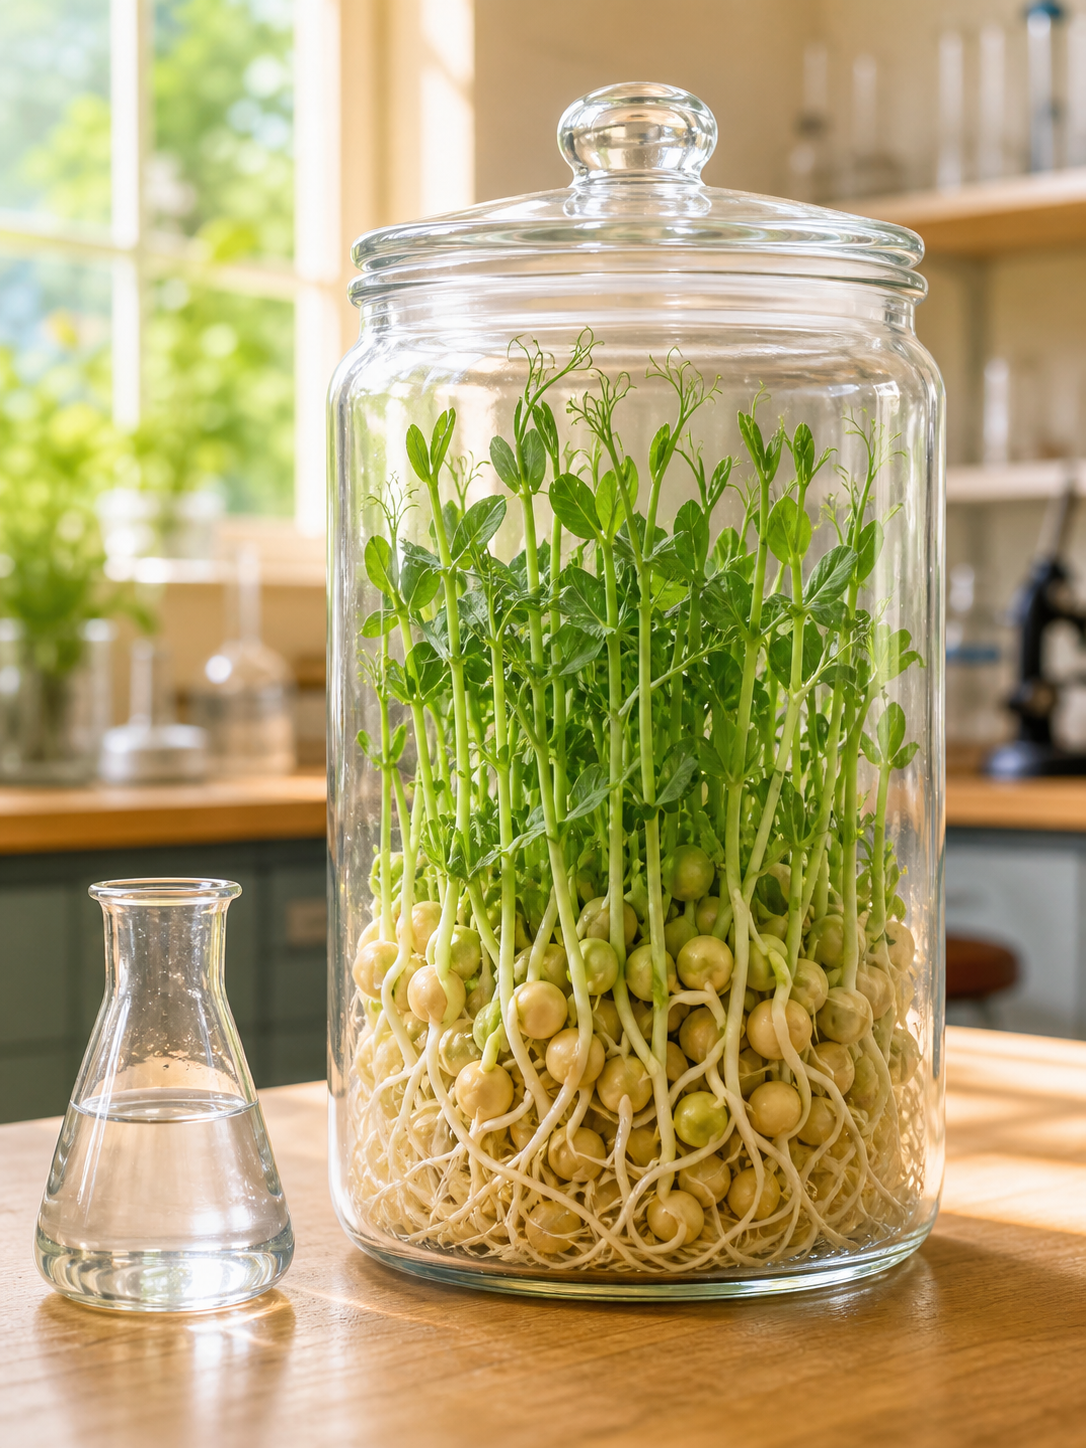
\includegraphics[width=0.46\linewidth]{images/book1/ai/g7-resp-peajar.png}

{\small The most unassuming respirer on the bench: a jar of
sprouting peas can exhaust its \omterm{def:g7:what-is-respiration:respiration}{oxygen} in a day.}
\end{omfigure}

\begin{remark}[Plants respire too]\label{rem:g7:what-is-respiration:plants}
\Cref{rem:g6:plants-are-producers:gas} said it in passing;
the jar proves it: a potted \omterm{def:g1:plants-around-us:plant}{plant} \emph{in the dark} lowers
its jar's \omterm{def:g7:what-is-respiration:respiration}{oxygen} and clouds \omterm{prop:g7:what-is-respiration:shown}{limewater} like any \omterm{def:g1:animals-around-us:animal}{animal}. In
daylight the \omterm{def:g5:food-webs:roles}{producers}' manufacture masks the effect ---
taking in far more \omterm{def:g7:what-is-respiration:respiration}{carbon dioxide} than \omterm{def:g7:what-is-respiration:respiration}{respiration} releases
--- but the \omterm{def:g7:what-is-respiration:respiration}{respiration} never stops. Green does not excuse a
\omterm{def:g5:first-look-at-cells:cell}{cell} from breathing-in-the-wide-sense; nothing living is
excused.
\end{remark}

\section{Why living things respire}

\begin{proposition}[Respiration powers the cells]\label{prop:g7:what-is-respiration:power}
The point of the swap is \emph{\omterm{prop:g3:balanced-diet:jobs}{energy}}. In every living
\omterm{def:g5:first-look-at-cells:cell}{cell}, \omterm{def:g4:journey-of-food:digestion}{nutrients} (\cref{def:g4:journey-of-food:digestion})
are slowly \emph{burned} with the \omterm{def:g7:what-is-respiration:respiration}{oxygen} \omterm{def:g7:what-is-respiration:respiration}{respiration}
brings: their \omterm{prop:g3:balanced-diet:jobs}{energy} is released for the \omterm{def:g5:first-look-at-cells:cell}{cell}'s work ---
contraction, building, commanding --- and \omterm{def:g7:what-is-respiration:respiration}{carbon dioxide}
is the burnt-out remainder, carted away.
\Cref{prop:g6:matter-from-food:losses}'s ``burned share''
was exactly this, seen from the ledger; here it is seen
from the \omterm{def:g5:first-look-at-cells:cell}{cell}.
\end{proposition}
\admitted

\begin{example}[The fire comparison, used honestly]\label{ex:g7:what-is-respiration:fire}
A candle flame also consumes \omterm{def:g7:what-is-respiration:respiration}{oxygen} and releases \omterm{def:g7:what-is-respiration:respiration}{carbon
dioxide} --- burning and \omterm{def:g7:what-is-respiration:respiration}{respiration} are genuinely the same
kind of chemistry. The differences matter as much: the
\omterm{def:g5:first-look-at-cells:cell}{cell}'s burning is slow, flameless, spread over thousands of
tiny steps, and its \omterm{prop:g3:balanced-diet:jobs}{energy} is captured for work rather than
lost as \omterm{def:g6:exploring-our-environment:conditions}{light} and scorch. \omterm{def:g7:what-is-respiration:respiration}{Respiration} is combustion
domesticated --- fire on a leash, in every \omterm{def:g5:first-look-at-cells:cell}{cell} you own.
\end{example}

\begin{example}[Reading demand]\label{ex:g7:what-is-respiration:demand}
Because the burning powers the work, demand tracks effort:
the sprinting child of \cref{ex:g4:breathing:running}
respires far faster than the reader in the armchair; the
germinating pea --- building a \omterm{def:g1:plants-around-us:plant}{plant} at full speed
(\cref{def:g2:from-seed-to-plant:germination}) --- respires
far faster than the dry, waiting \omterm{def:g2:from-seed-to-plant:seed}{seed} beside it, whose
\omterm{def:g7:what-is-respiration:respiration}{respiration} idles near zero for years. \omterm{def:g7:what-is-respiration:respiration}{Respiration} is the
engine note of life: loud in effort and growth, a whisper
in dormancy, silent only in death.
\end{example}

\section{Respiration in every habitat}

\begin{proposition}[One need, many surroundings]\label{prop:g7:what-is-respiration:habitats}
Every \omterm{def:g6:exploring-our-environment:components}{living thing} must get its \omterm{def:g7:what-is-respiration:respiration}{oxygen} \emph{from its
surroundings} --- and surroundings differ. Air is
oxygen-rich; water holds far less, dissolved
(\cref{exo:g4:breathing:11} met the consequence); \omterm{def:g6:decomposers-and-soil:soil}{soil} and
mud hold less still. Where and how a \omterm{def:g6:exploring-our-environment:components}{living thing} lives is
therefore shaped by how it solves its \omterm{def:g7:what-is-respiration:respiration}{oxygen} problem ---
the subject of the next two chapters, for \omterm{def:g1:animals-around-us:animal}{animals}'
equipment (\cref{ch:g7:how-animals-breathe}) and for
water's economy (\cref{ch:g7:oxygen-in-the-water}).
\end{proposition}
\admitted

\begin{method}[Testing a respiration question]\label{met:g7:what-is-respiration:test}
To test any claim about \omterm{def:g7:what-is-respiration:respiration}{respiration} (``\omterm{prop:g3:flowers-fruits-seeds:transform}{seeds} respire
faster warm'', ``the pond mud respires''):
\begin{enumerate}
  \item close the subject in a container, with an \omterm{def:g7:what-is-respiration:respiration}{oxygen}
        probe or a \omterm{prop:g7:what-is-respiration:shown}{limewater} trap;
  \item build the twin control --- same container,
        subject absent or lifeless;
  \item vary one condition at a time, if the claim names
        one (warmth, dampness, dark);
  \item read the verdict in the difference: \omterm{def:g7:what-is-respiration:respiration}{oxygen} fallen,
        \omterm{prop:g7:what-is-respiration:shown}{limewater} clouded --- against the control's
        stillness.
\end{enumerate}
\end{method}

\begin{example}[The method on a cold seed]\label{ex:g7:what-is-respiration:coldseed}
Claim: germinating peas respire more slowly in the cold.
Two jars of sprouting peas, one at room warmth, one in the
fridge; \omterm{prop:g7:what-is-respiration:shown}{limewater} traps on both; a lifeless third as
control. Next day: the warm jar's \omterm{prop:g7:what-is-respiration:shown}{limewater} is milky, the
cold jar's barely misted, the control's clear. Verdict:
\omterm{def:g7:what-is-respiration:respiration}{respiration} runs with the peas' working pace ---
\cref{prop:g6:decomposers-and-soil:speed}'s
conditions-rule, measured in gas.
\end{example}

\section{Exercises}

\begin{exercise}[$\star$]\label{exo:g7:what-is-respiration:1}
Define \omterm{def:g7:what-is-respiration:respiration}{respiration}, and distinguish it from \omterm{def:g7:what-is-respiration:respiration}{breathing}.
\end{exercise}

\begin{exercise}[$\star$]\label{exo:g7:what-is-respiration:2}
Name the two bench tests that reveal \omterm{def:g7:what-is-respiration:respiration}{respiration}, and what
each shows.
\end{exercise}

\begin{exercise}[$\star$]\label{exo:g7:what-is-respiration:3}
Why does every \omterm{def:g7:what-is-respiration:respiration}{respiration} experiment need a lifeless
control container?
\end{exercise}

\begin{exercise}[$\star$]\label{exo:g7:what-is-respiration:4}
What is the point of \omterm{def:g7:what-is-respiration:respiration}{respiration}, by
\cref{prop:g7:what-is-respiration:power}? What is \omterm{def:g7:what-is-respiration:respiration}{carbon
dioxide}, in that account?
\end{exercise}

\begin{exercise}[$\star$]\label{exo:g7:what-is-respiration:5}
List five very different \omterm{def:g6:exploring-our-environment:components}{living things} shown respiring in
\cref{ex:g7:what-is-respiration:gallery}.
\end{exercise}

\begin{exercise}[$\star$]\label{exo:g7:what-is-respiration:6}
How can a \omterm{def:g1:plants-around-us:plant}{plant} be shown to respire, given that daylight
masks the effect?
\end{exercise}

\begin{exercise}[$\star\star$]\label{exo:g7:what-is-respiration:7}
Give two honest likenesses and two honest differences
between a candle's burning and a \omterm{def:g5:first-look-at-cells:cell}{cell}'s \omterm{def:g7:what-is-respiration:respiration}{respiration}.
\end{exercise}

\begin{exercise}[$\star\star$]\label{exo:g7:what-is-respiration:8}
Rank by \omterm{def:g7:what-is-respiration:respiration}{respiration} rate, with reasons: a dry pea, a
germinating pea, a sprinting child, a reading child.
\end{exercise}

\begin{exercise}[$\star\star$]\label{exo:g7:what-is-respiration:9}
A sealed jar of sprouting peas goes overnight; a candle
lowered in next morning goes straight out. Explain with
this chapter --- and say what the \omterm{prop:g7:what-is-respiration:shown}{limewater} trap would
have shown meanwhile.
\end{exercise}

\begin{exercise}[$\star\star$]\label{exo:g7:what-is-respiration:10}
Design, by \cref{met:g7:what-is-respiration:test}, the
experiment for: ``living \omterm{def:g6:decomposers-and-soil:soil}{soil} respires; baked lifeless
\omterm{def:g6:decomposers-and-soil:soil}{soil} does not.''
\end{exercise}

\begin{exercise}[$\star\star$]\label{exo:g7:what-is-respiration:11}
Why does a grain store's manager fear damp grain heaps
warming by themselves? Connect
\cref{ex:g7:what-is-respiration:demand} and the compost
heap's warmth
(\cref{ex:g6:decomposers-and-soil:compost}).
\end{exercise}

\begin{exercise}[$\star\star\star$]\label{exo:g7:what-is-respiration:12}
``\omterm{def:g4:breathing:movements}{Breathing} is behavior; \omterm{def:g7:what-is-respiration:respiration}{respiration} is chemistry; the
first serves the second.'' Defend each clause with one
observation from this chapter or
\cref{ch:g4:breathing}.
\end{exercise}

\section{Problem: The Sealed Jars}

\begin{problem}[{Weekend problem --- six jars, two
mysteries, one gas swap}]\label{pb:g7:what-is-respiration:1}
For the science fair, the class prepares six sealed jars,
each with an \omterm{def:g7:what-is-respiration:respiration}{oxygen} probe and a \omterm{prop:g7:what-is-respiration:shown}{limewater} trap: A ---
pebbles; B --- dry peas; C --- germinating peas; D --- a
mouse (with food, water, and for a few hours only, under
the teacher's watch); E --- a green \omterm{def:g1:plants-around-us:plant}{plant} in the \omterm{def:g6:exploring-our-environment:conditions}{light}; F
--- the same kind of \omterm{def:g1:plants-around-us:plant}{plant} in a dark box.

\medskip\noindent\textbf{Part I --- Predictions.}
\begin{enumerate}
  \item Predict A's readings, and state A's job in the
        experiment.
  \item Predict B and C, and explain the difference
        although both jars hold ``the same'' peas.
  \item Predict D, and say why the teacher limits the
        hours.
  \item E and F hold identical \omterm{def:g1:plants-around-us:plant}{plants}. Predict each jar's
        \omterm{def:g7:what-is-respiration:respiration}{oxygen} trend, and reconcile the difference using
        \cref{rem:g7:what-is-respiration:plants}.
\end{enumerate}

\medskip\noindent\textbf{Part II --- Results and readings.}
\begin{enumerate}[resume]
  \item The morning's data match the predictions --- except
        a classmate is amazed that F's \omterm{def:g1:plants-around-us:plant}{plant} ``breathes
        like an \omterm{def:g1:animals-around-us:animal}{animal}''. Set out what F actually shows,
        and what E hides.
  \item C's \omterm{def:g7:what-is-respiration:respiration}{oxygen} fell three times faster than B's per
        gram of peas. Translate the factor of three into
        \cref{ex:g7:what-is-respiration:demand}'s terms.
  \item D's \omterm{prop:g7:what-is-respiration:shown}{limewater} clouded fastest of all. Give the
        chain --- from the mouse's warm, moving body to the
        milky liquid --- in four steps.
  \item Name the single conclusion all of B, C, D and F
        support, in one sentence beginning ``Every \omterm{def:g6:exploring-our-environment:components}{living
        thing}\dots''.
\end{enumerate}

\medskip\noindent\textbf{Part III --- Pressing further.}
\begin{enumerate}[resume]
  \item A seventh jar is proposed: mushroom slices. Predict
        its readings, and say which kingdom-level point of
        \cref{ex:g7:what-is-respiration:gallery} it would
        add.
  \item The fair's visitors ask why jar C matters to
        farmers. Answer with the granary of
        \cref{exo:g7:what-is-respiration:11}.
  \item An eighth jar: pond water with its mud. The \omterm{def:g7:what-is-respiration:respiration}{oxygen}
        falls overnight. Who in the jar is respiring, and
        why does the finding matter for
        \cref{ch:g7:oxygen-in-the-water}'s question?
  \item Close the fair's poster with the chapter's
        distinction: which jars showed \emph{\omterm{def:g7:what-is-respiration:respiration}{breathing}},
        and which showed \emph{\omterm{def:g7:what-is-respiration:respiration}{respiration}}? (Careful ---
        one word covers them all.)
\end{enumerate}
\end{problem}
